\section{Evaluation}
\label{sec:eval}

\begin{figure*}[t]
  \centering
  \setlength{\abovecaptionskip}{0pt}
  \setlength{\belowcaptionskip}{0pt}
  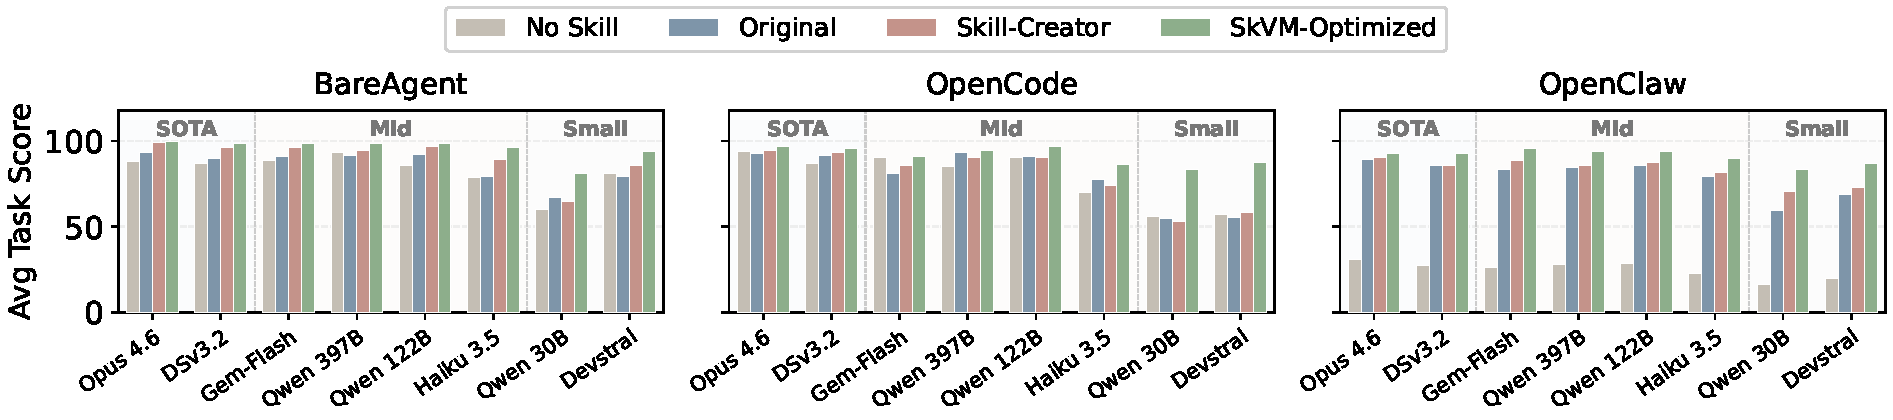
\includegraphics[width=\textwidth]{figures/e1_overview.pdf}
  \caption{Average task score by skill variant.
    Four variants are compared across eight models and three harnesses:
    No Skill, Original, Skill-Creator, and \sys-Optimized.
    Tier boundaries (SOTA / Mid / Small) are shaded.
    \sys-Optimized skills consistently achieve the highest scores, with the
    largest absolute gains for weaker models and on OpenClaw.}
  \label{fig:e1_overview}
\end{figure*}

\subsection{Setup}
\label{sec:eval:setup}

\heading{Benchmark.}
We select and extend existing skill benchmarks, including SkillsBench~\cite{li2026skillsbench} and PinchBench~\cite{pinchbench}, covering diverse agent tasks spanning code generation, data analysis, document creation, and system administration.
Each task is paired with at least one skill sourced from mainstream skill sources: Anthropic-skills~\cite{anthropic-skills-repo}, OpenClaw skills~\cite{openclaw}, and skills.sh~\cite{skillssh}.
We employ an automated evaluation suite comprising static analysis and LLM-based assessment against predefined criteria~\cite{zhu2024swebench, zheng2023llmasjudge}.

\heading{Models.}
We evaluate \sys across eight models spanning three capability tiers to comprehensively assess its effectiveness across varying model capacities.
\emph{SOTA}: claude-opus-4.6~\cite{claude4_6_opus}, deepseek-v3.2~\cite{deepseek2025v3}.
\emph{Mid-tier}: gemini-3-flash~\cite{gemini_flash}, qwen3.5-397b~\cite{qwen3_5_397b}, qwen3.5-122b~\cite{qwen3_5_122b}, claude-3.5-haiku~\cite{claude3_5_haiku}.
\emph{Small}: qwen3-30b~\cite{qwen3_30b}, devstral-small~\cite{devstral_small_2507}.

\heading{Baselines.}
We compare \sys against three baselines.
\emph{No Skill}: the agent executes without any skill loaded.
\emph{Original}: the original skill.
\emph{Skill-Creator}: the skill optimized by Anthropic's Skill-Creator~\cite{anthropic-skill-creator} using claude-opus-4.6.

\heading{Harnesses.}
We select three different open-source agent harnesses to evaluate \sys performance across diverse execution environments.
Each harness offers distinct functionality:
\emph{BareAgent}: a minimal harness that injects the compiled skill
directly into the system prompt without additional abstraction layers.
\emph{OpenCode}~\cite{opencode}: a full-featured code agent harness with batch tool
dispatch capabilities and a rich tool set for code execution.
\emph{OpenClaw}~\cite{openclaw}: a general-purpose agent harness with integrated functional
modules designed to support complex multi-step task execution.

\heading{Methodology.}
We first profile the primitive capabilities of different models, and then apply \sys's AOT and JIT compilation to generate optimized skill variants tailored to each model.
To support the compiled skill artifacts, we extend the agent harnesses with custom loading and management mechanisms that enable \sys's optimizations.
For each task, we generate five diverse input instances and measure the average task completion rate, token consumption, and end-to-end execution latency.
All experiments are conducted on a Mac Mini M4 with 16GB memory.

\begin{figure}[t]
  \setlength{\abovecaptionskip}{3pt}
  \setlength{\belowcaptionskip}{-5pt}
  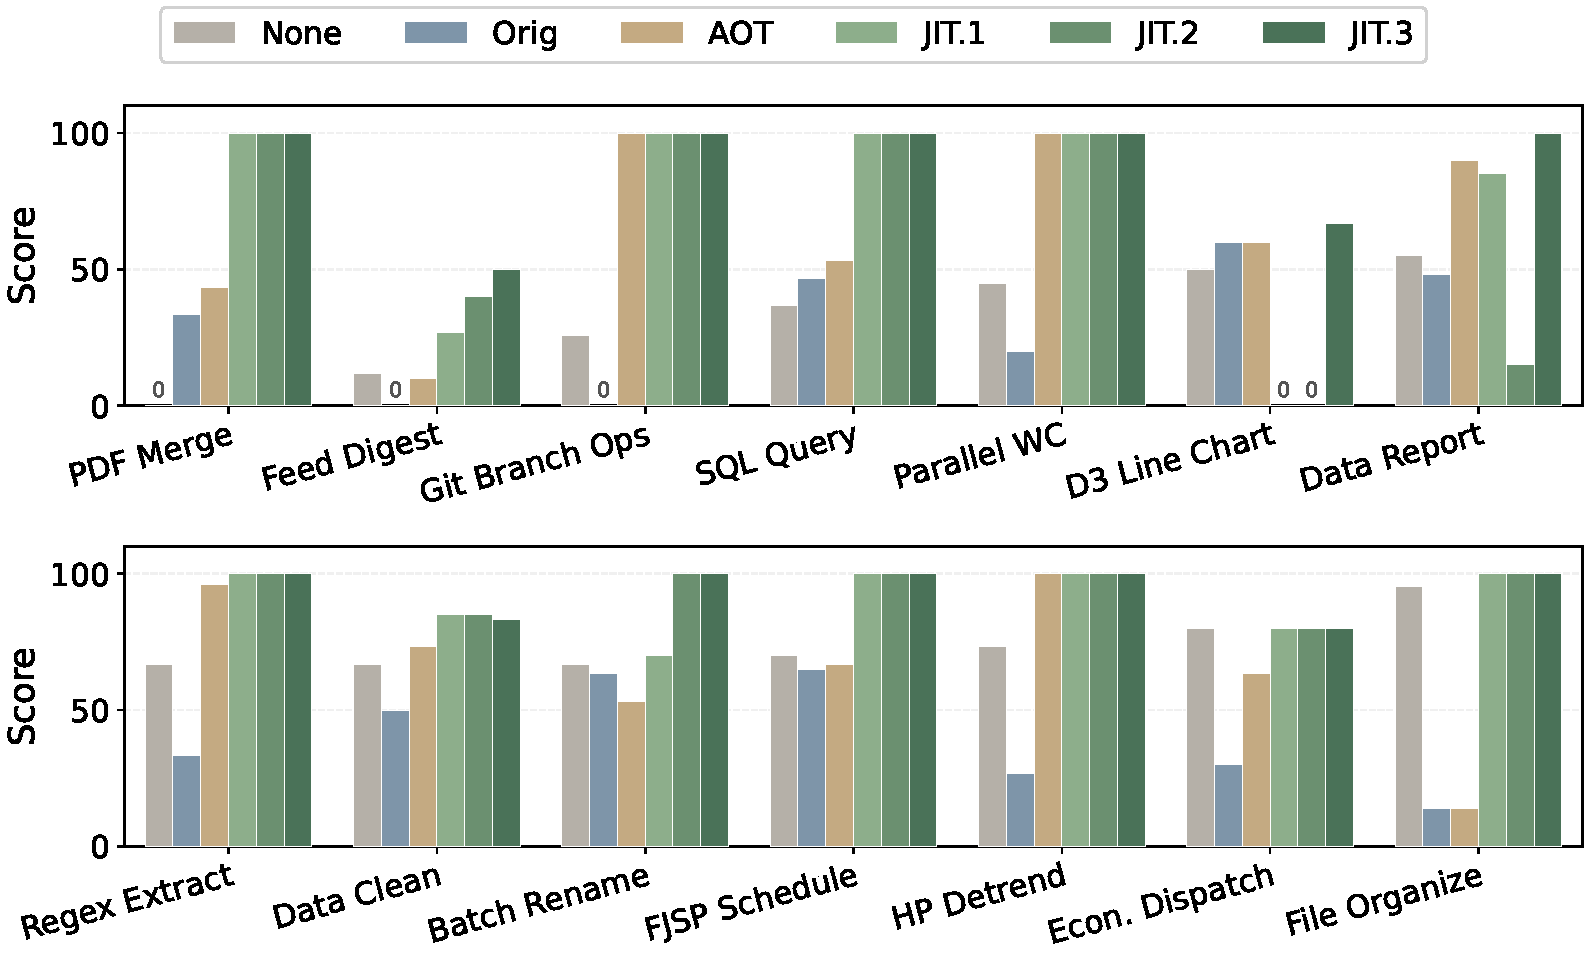
\includegraphics[width=\columnwidth]{figures/e6_skill_progression_bar.pdf}
  \caption{Staged optimization breakdown across 14 skill categories.
  Each group shows scores at six stages: no skill, original skill,
  AOT-compiled skill, and skills optimized in three JIT rounds. }
  \label{fig:e6}
\end{figure}

\subsection{Skill Compilation Effectiveness}
\label{sec:eval:e1}

We first evaluate \sys's effectiveness in improving task completion rates.
We compare \sys-optimized skills against unoptimized baseline skills across different tasks, models, and agent harnesses.
For \sys, the primary gains stem from capability-based compilation and JIT optimization.
Figure~\ref{fig:e1_heatmap} presents compilation effectiveness across eight models and three harnesses.
Cell values represent task completion rates after \sys optimization, while cell color indicates the score improvement (green) or regression (red) relative to unoptimized baseline skills.

Figure~\ref{fig:e1_heatmap} demonstrates \sys's optimization effectiveness (compared with original skills) across diverse models and agent harnesses.
Weaker models benefit more substantially from \sys optimization.
This finding indicates that for most agent tasks, weaker models possess sufficient capability for the logical components but lack proficiency in non-logical aspects, such as generating complex JSON structures or managing environment dependencies.
\sys's compilation optimization addresses these gaps through primitive capability refinement, 
thereby improving overall task completion rates.
For stronger models, improvements are more modest, as these models already handle tasks competently; 
\sys optimization primarily reduces token consumption and execution latency.
Figure~\ref{fig:e1_overview} aggregates average task scores across all four skill variants
for each model and harness.
\sys-optimized skills achieve the highest scores on every model--harness combination.
The improvement over the Skill-Creator baseline grows with decreasing model capability:
on BareAgent, \sys-optimized skills improve over Skill-Creator by 25\% for qwen3-30b and 10\% for devstral-small.
In terms of regressions, \sys-compiled skills reduce task completion rates on only 4.5\% of tasks, compared with 15\% for the original skills.
Using the original skill, OpenCode and OpenClaw differ by up to 13 points,
depending on the model, which shows that harness behavior alone materially changes outcomes.
\sys optimization raises scores on both harnesses and reduces this cross-harness gap to at most 5 points.


\subsection{Staged Optimization Breakdown}
\label{sec:eval:e6}

Figure~\ref{fig:e6} breaks down the contribution of each optimization stage
across 14 skill categories on Qwen3-30B with BareAgent.
Each group shows scores at six stages: no skill, original skill,
AOT-compiled skill, and up to three rounds of JIT optimization.
Tasks used in each round are of the same type but differ in contents.

In 11 of 14 categories, the original skill performs worse than using no skill.
After \sys's AOT compilation, the average task score improves by 88\%.
JIT optimization identifies additional capability defects that were not exposed during AOT compilation,
further improving performance.
After one JIT round, 8 of 14 skills achieve full scores on the
evaluation tasks, and after three rounds, 10 of 14 do so.

JIT optimization can introduce regressions.
For example, in the Line Chart task, the JIT compiler added an example file to the skill,
but the file was too long and triggered parsing errors, which reduced the score.
After three rounds of revision guided by prior failure logs, the JIT compiler eventually fixed this issue.

\subsection{Token and Cost Efficiency with Compilation}
\label{sec:eval:e2}

Beyond improving task success rates, \sys provides substantial cost benefits for SOTA LLMs by reducing token consumption.
LLMs can correct execution errors through iterative agent loops, refining actions based on environment feedback.
Therefore, even when tasks eventually succeed, this approach may incur substantial token waste.
Figure~\ref{fig:e2_scatter} shows how task success rates and token costs vary across different model tiers and harnesses after \sys compilation.

Our evaluation reveals that for most models and harness combinations, \sys compilation simultaneously improves task success and reduces token consumption.
For the strongest model and weakest harness pairing (DS-v3.2 + BareAgent), we observe token savings approaching 40\%.
This improvement arises because agent loops incur interaction overhead when correcting environment-related and tool-invocation errors; multiple retries are often required.
By employing JIT compilation, \sys enables models to avoid these error paths entirely, eliminating redundant interactions and saving substantial tokens.

For weaker models, \sys may occasionally consume additional tokens.
This occurs because \sys improves task completion rates, leading to longer agent execution traces compared to the baseline skill, resulting in modest token increases in edge cases.


\begin{figure}[t]
  \centering
  \setlength{\abovecaptionskip}{5pt}
  \setlength{\belowcaptionskip}{-3pt}
  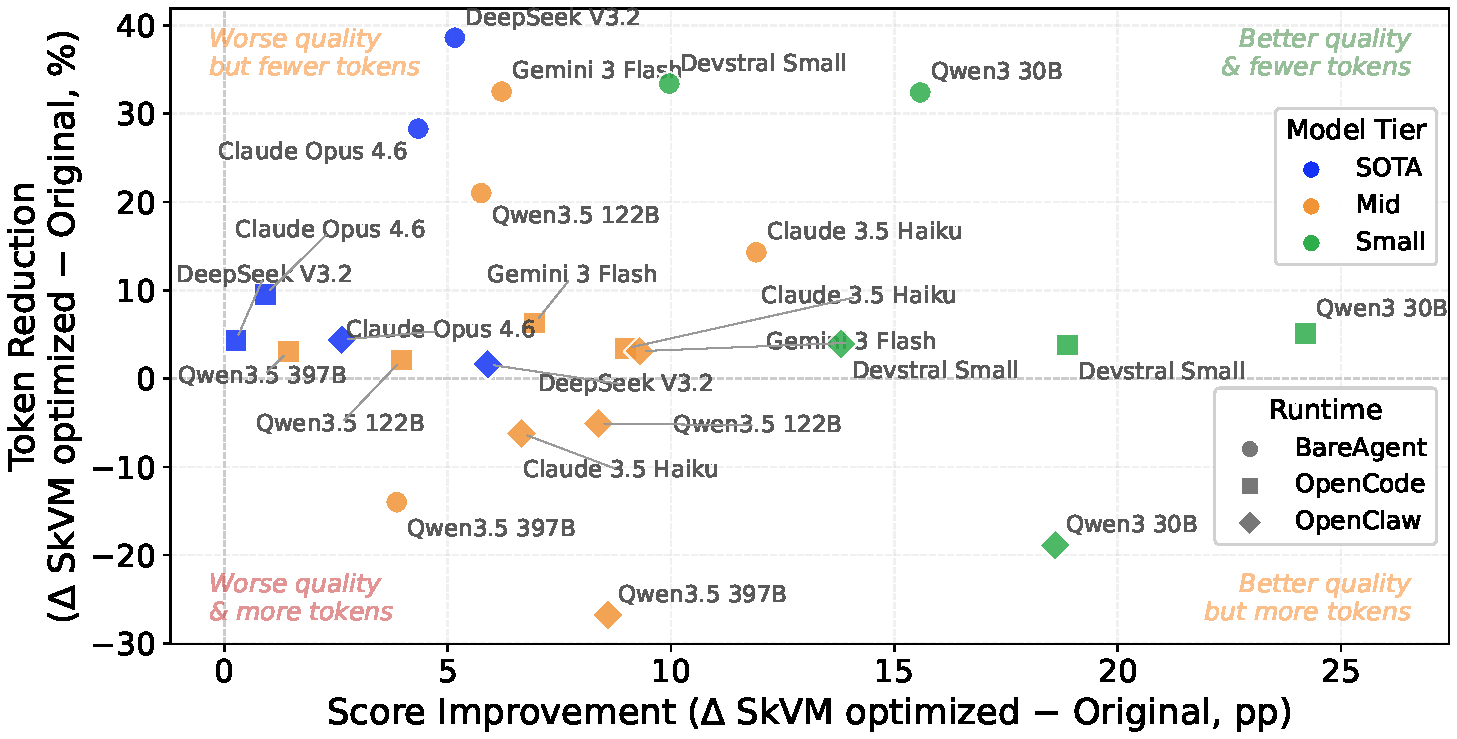
\includegraphics[width=\columnwidth]{figures/e2_scatter.pdf}
  \caption{Score gain vs.\ token savings for \sys
    optimization over the Original baseline. Each point is a
    (model, harness) pair. Color = model tier, shape = harness.
    Most points land in the upper-right quadrant: better
    quality \emph{and} fewer tokens.}
  \label{fig:e2_scatter}
\end{figure}

\begin{figure}[t]
  \centering
  \setlength{\abovecaptionskip}{5pt}
  \setlength{\belowcaptionskip}{0pt}
  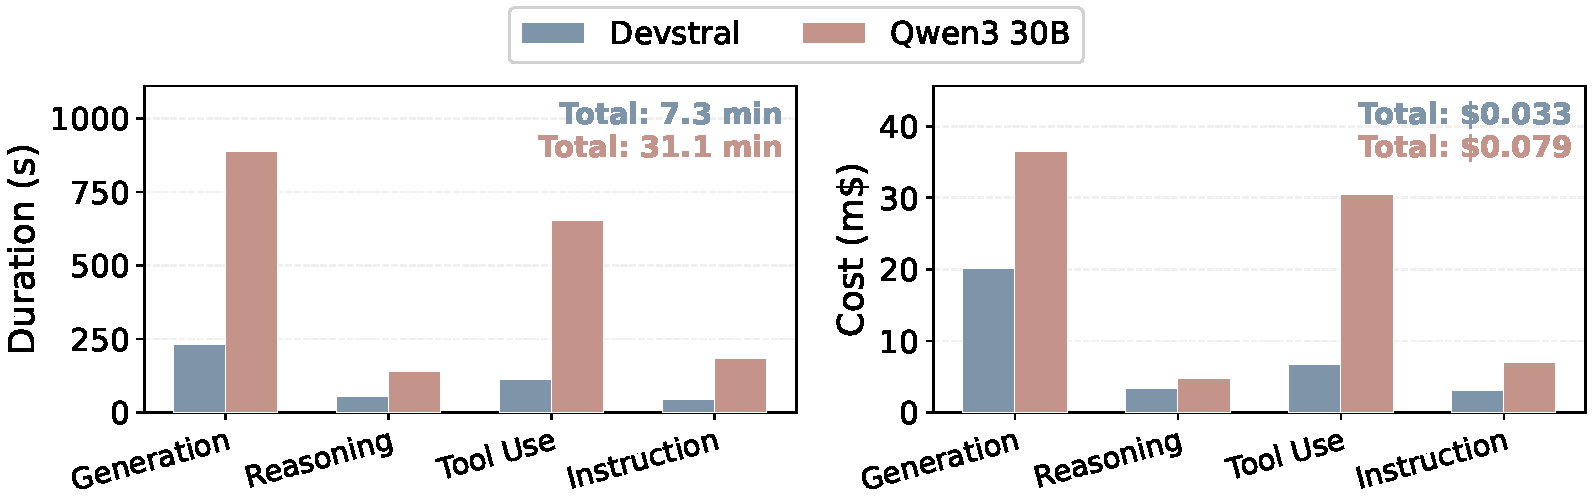
\includegraphics[width=\columnwidth]{figures/profiling_cost.pdf}
  \caption{Per-category breakdown of capability profiling
    overhead for two small models. Left: duration in seconds.
    Right: cost in millidollars.}
  \label{fig:profiling_cost}
\end{figure}

\begin{figure}[t]
\centering
\setlength{\abovecaptionskip}{3pt}
\setlength{\belowcaptionskip}{0pt}
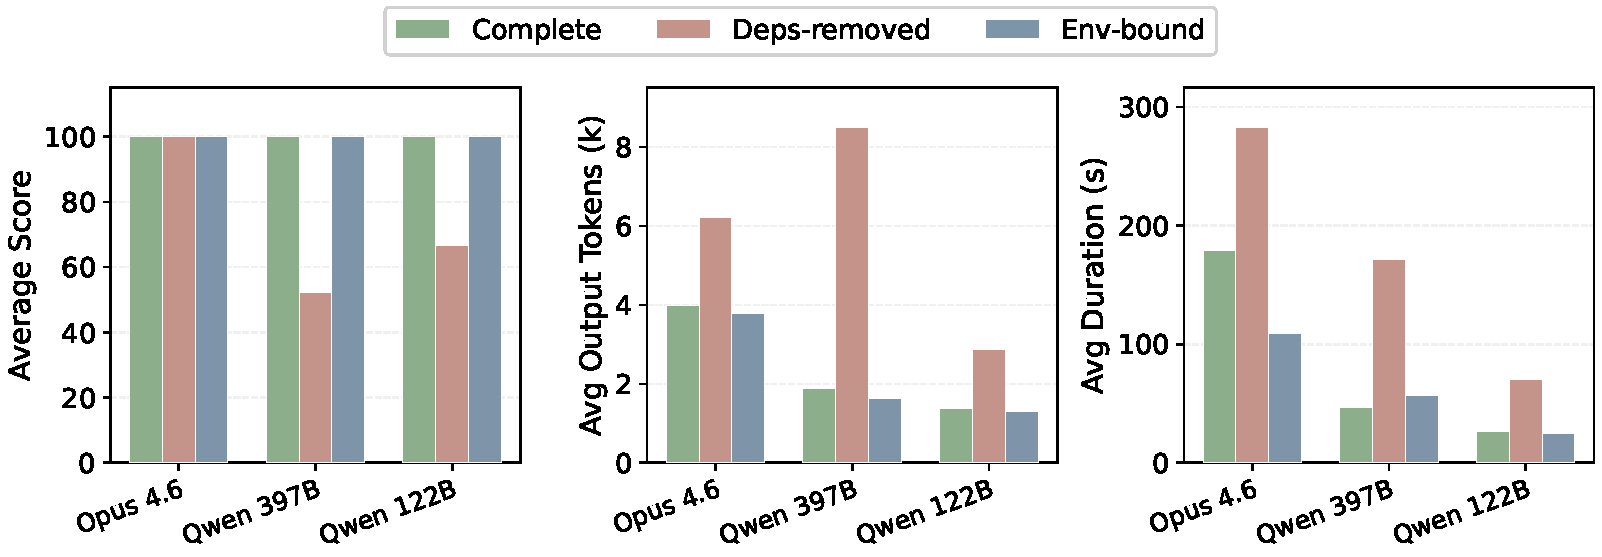
\includegraphics[width=\columnwidth]{figures/e3_env_adaptation.pdf}
\caption{Environment binding restores correctness, token
  efficiency, and execution speed. From left to right: average
  score, average token use, and average duration across two
  tasks per model. Env-bound performance returns to
  complete-environment levels for all three models.}
\label{fig:e3}
\end{figure}

\begin{figure*}[t]
  \centering
  \setlength{\abovecaptionskip}{3pt}
  \setlength{\belowcaptionskip}{0pt}
  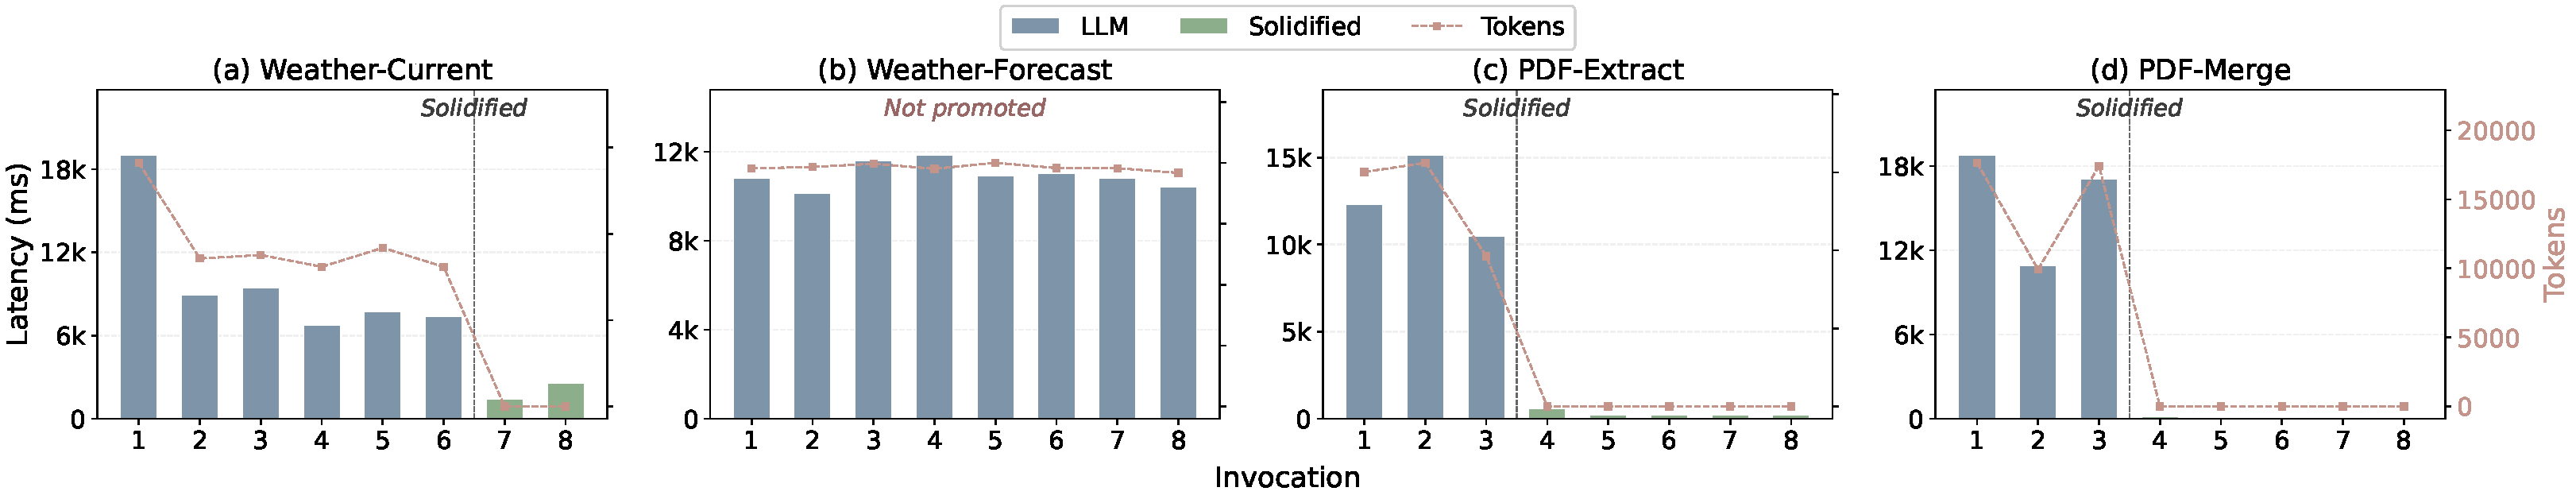
\includegraphics[width=\textwidth]{figures/e5_jit_demo.pdf}
  \caption{Code solidification across four cases. Blue bars
    show LLM inference latency, green bars show solidified
    execution. The dashed line marks the promotion point.
    Weather-forecast never promotes because the runtime
    model's code patterns diverge from the AOT prediction,
    validating the promotion gate as a safety mechanism.}
  \label{fig:e5_jit}
\end{figure*}



\subsection{Overhead of Target Profiling}
\label{sec:eval:profiling}

Capability-based compilation requires profiling the target once
to build its capability profile (\S\ref{sec:compiler:cap}).
This profiling is a one-time cost per (model, harness) pair,
and the results are cached and reused for all subsequent
skill compilations on the same target.
We measure this overhead on two small models, devstral-small and qwen3-30b. 

Figure~\ref{fig:profiling_cost} shows the per-category breakdown
of profiling duration and cost.
A full profile across all primitive capabilities completes in
7.3 minutes for devstral-small and 31.1 minutes for qwen3-30b,
costing \$0.033 and \$0.079 respectively.

\subsection{Evaluating Environment Binding}
\label{sec:eval:e3}

The preceding two experiments conducted testing in fully provisioned environments. However, in real-world skill scenarios, missing environment dependencies during agent execution are commonplace. Resolving such environmental issues presents significant challenges for weaker LLMs, frequently resulting in skill execution failures. \sys addresses this through an environment binding mechanism in its AOT compilation phase. This mechanism shifts environment dependency installation from the LLM execution phase to pre-execution preprocessing, allowing the LLM to focus solely on skill logic.

Figure~\ref{fig:e3} demonstrates the performance of different models across three environmental configurations: complete, with environment binding, and with missing dependencies.
Stronger models such as claude-opus-4.6 can autonomously recover from missing dependencies, but at the cost of increased token consumption.
For weaker models such as qwen3.5-122b, missing dependencies lead to execution failures.
Environment binding fully restores execution correctness and substantially reduces token consumption.

\subsection{Evaluating Concurrency Extraction}
\label{sec:eval:e4}

\sys extracts more parallelism opportunities within skills and improves efficiency.
We evaluate three parallelism types: data-level parallelism (DLP),
instruction-level parallelism (ILP), and thread-level parallelism (TLP).
DLP applies when instructions within a single skill batch-process large
amounts of independent data. ILP applies when multiple independent instructions
or code segments within a skill can execute concurrently. TLP applies when
multiple independent sub-agents run within a skill, each processing
self-contained subtasks without cross-dependencies. Figure~\ref{fig:e4}
demonstrates \sys's performance improvements across these three parallelism
types.

Experimental results show that \sys's parallelism extraction strategy
achieves up to 3.2$\times$ end-to-end speedup. TLP yields the largest
average improvements because its coarser-grain parallelism produces more
pronounced optimization effects. ILP, operating at the instruction level,
reduces both execution time and the number of LLM invocations. DLP gains
stem purely from data parallelism, such that the performance
improvement scales directly with the degree of data parallelism.
We also observe inherent variability in agent execution due to LLM throughput
fluctuations and varying numbers of agent loop iterations. Consequently,
timing variations within a reasonable range are acceptable.

\begin{figure}[t]
\centering
\setlength{\abovecaptionskip}{5pt}
\setlength{\belowcaptionskip}{-5pt}
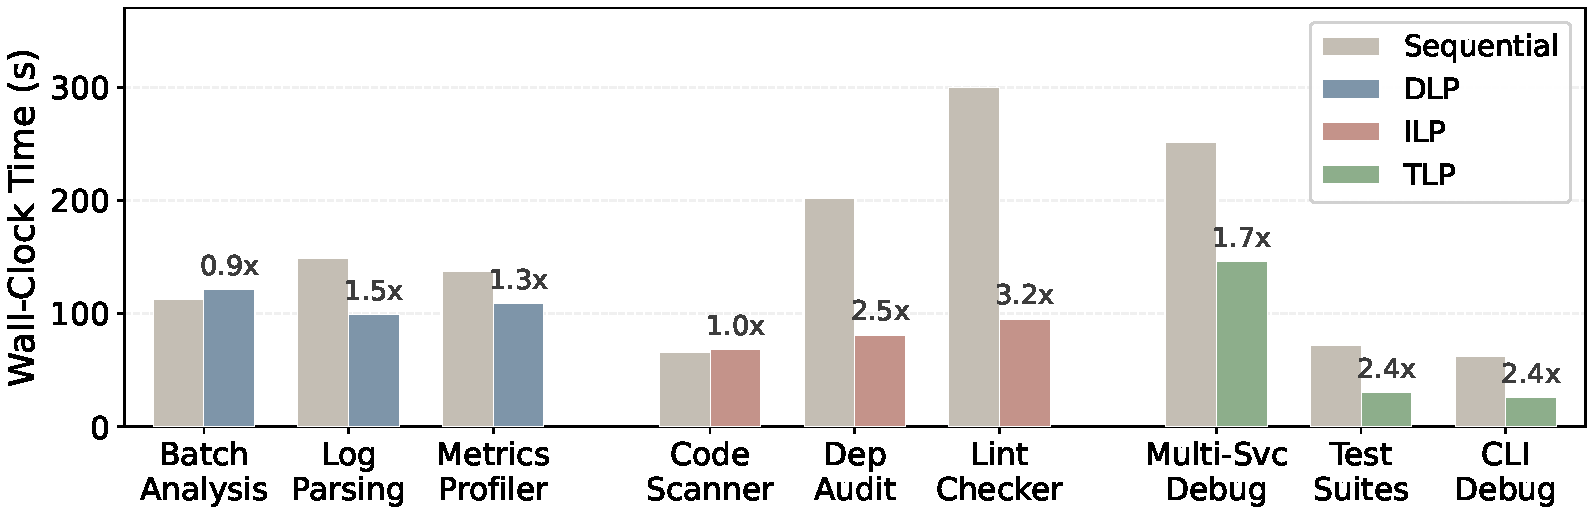
\includegraphics[width=\columnwidth]{figures/e4_parallelism.pdf}
\caption{Performance of different parallelization strategies across eight tasks.
  Bars show sequential, DLP, ILP, and TLP execution.}
\label{fig:e4}
\end{figure}

\subsection{Evaluating Code Solidification}
\label{sec:eval:e5}

We further analyze whether adopting code solidification
mechanisms from JIT optimization can accurately identify
reusable code segments and improve agent execution
efficiency. As shown in Figure~\ref{fig:e5_jit}, we conduct
a detailed analysis on two canonical skills (weather,
document-pdf).
For the two PDF tasks, despite variations in task inputs, the LLM-generated code matches the code signature. Therefore, \sys can apply JIT compilation optimization, directly generating solidified code using the template and input parameters. 
For PDF-extract tasks, JIT optimization reduces execution time from
10,469--15,116\,ms to 206--568\,ms, achieving a 19--50$\times$ speedup.
For the two weather tasks, weather-current requires external weather API calls,
the speedup is bounded by network latency, reducing execution time from 9,000\,ms
to 2,000\,ms, yielding a 5$\times$ improvement. 
In contrast, weather-forecast uses more flexible formats,
so the generated code structures diverge from the code signature and fail to match.
Consequently, all eight invocations rely on
LLM generation to avoid invoking incorrect code.


If solidified code execution causes task failure, \sys's safety mechanism
triggers fallback, re-enabling LLM code generation to ensure correctness.

